\paragraph{Function detouring}
\begin{figure}[!htbp]
	\centering
	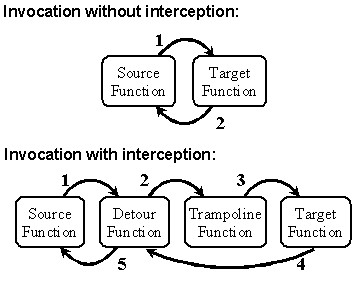
\includegraphics[scale=0.7]{sections/background/attacks/fig_detours.png}
	\caption{This figure shows the change in control flow of a detoured function \cite{detours}}
	\label{fig:detours}
\end{figure}


Function detouring has been greatly simplified by the Detours\cite{msdetours} library of Microsoft, but can also be achieved by memory modification with \syscall{WriteProcessMemory} or assembly code. Figure \ref{fig:detours} shows the difference between a function before and after detouring. The function call at the top shows a invocation without interception. The source function calls the target function without any indirection and after the code of the target function has been executed, returns to the calling source function. Detouring makes use of this structure by placing a detour and a trampoline function in between these calls. The source function will now use an indirect call to the target function, by first calling the detour part, which gives space to execute arbitrary code. To do that, a \syscall{jmp} instruction is placed at the beginning of the function, and the original instructions are saved and copied to the trampoline function. After that, the detour function continues with the trampoline function, which executes the copied instructions and ensures that the target function works as if there was no detour placed. Finally, the whole function stack will return, this time skipping the trampoline function, as it was just used to hold the copied instructions.